% Options for packages loaded elsewhere
\PassOptionsToPackage{unicode}{hyperref}
\PassOptionsToPackage{hyphens}{url}
%
\documentclass[
]{article}
\usepackage{lmodern}
\usepackage{amssymb,amsmath}
\usepackage{ifxetex,ifluatex}
\ifnum 0\ifxetex 1\fi\ifluatex 1\fi=0 % if pdftex
  \usepackage[T1]{fontenc}
  \usepackage[utf8]{inputenc}
  \usepackage{textcomp} % provide euro and other symbols
\else % if luatex or xetex
  \usepackage{unicode-math}
  \defaultfontfeatures{Scale=MatchLowercase}
  \defaultfontfeatures[\rmfamily]{Ligatures=TeX,Scale=1}
\fi
% Use upquote if available, for straight quotes in verbatim environments
\IfFileExists{upquote.sty}{\usepackage{upquote}}{}
\IfFileExists{microtype.sty}{% use microtype if available
  \usepackage[]{microtype}
  \UseMicrotypeSet[protrusion]{basicmath} % disable protrusion for tt fonts
}{}
\makeatletter
\@ifundefined{KOMAClassName}{% if non-KOMA class
  \IfFileExists{parskip.sty}{%
    \usepackage{parskip}
  }{% else
    \setlength{\parindent}{0pt}
    \setlength{\parskip}{6pt plus 2pt minus 1pt}}
}{% if KOMA class
  \KOMAoptions{parskip=half}}
\makeatother
\usepackage{xcolor}
\IfFileExists{xurl.sty}{\usepackage{xurl}}{} % add URL line breaks if available
\IfFileExists{bookmark.sty}{\usepackage{bookmark}}{\usepackage{hyperref}}
\hypersetup{
  pdftitle={DataProcessingDocument},
  hidelinks,
  pdfcreator={LaTeX via pandoc}}
\urlstyle{same} % disable monospaced font for URLs
\usepackage[margin=1in]{geometry}
\usepackage{color}
\usepackage{fancyvrb}
\newcommand{\VerbBar}{|}
\newcommand{\VERB}{\Verb[commandchars=\\\{\}]}
\DefineVerbatimEnvironment{Highlighting}{Verbatim}{commandchars=\\\{\}}
% Add ',fontsize=\small' for more characters per line
\usepackage{framed}
\definecolor{shadecolor}{RGB}{248,248,248}
\newenvironment{Shaded}{\begin{snugshade}}{\end{snugshade}}
\newcommand{\AlertTok}[1]{\textcolor[rgb]{0.94,0.16,0.16}{#1}}
\newcommand{\AnnotationTok}[1]{\textcolor[rgb]{0.56,0.35,0.01}{\textbf{\textit{#1}}}}
\newcommand{\AttributeTok}[1]{\textcolor[rgb]{0.77,0.63,0.00}{#1}}
\newcommand{\BaseNTok}[1]{\textcolor[rgb]{0.00,0.00,0.81}{#1}}
\newcommand{\BuiltInTok}[1]{#1}
\newcommand{\CharTok}[1]{\textcolor[rgb]{0.31,0.60,0.02}{#1}}
\newcommand{\CommentTok}[1]{\textcolor[rgb]{0.56,0.35,0.01}{\textit{#1}}}
\newcommand{\CommentVarTok}[1]{\textcolor[rgb]{0.56,0.35,0.01}{\textbf{\textit{#1}}}}
\newcommand{\ConstantTok}[1]{\textcolor[rgb]{0.00,0.00,0.00}{#1}}
\newcommand{\ControlFlowTok}[1]{\textcolor[rgb]{0.13,0.29,0.53}{\textbf{#1}}}
\newcommand{\DataTypeTok}[1]{\textcolor[rgb]{0.13,0.29,0.53}{#1}}
\newcommand{\DecValTok}[1]{\textcolor[rgb]{0.00,0.00,0.81}{#1}}
\newcommand{\DocumentationTok}[1]{\textcolor[rgb]{0.56,0.35,0.01}{\textbf{\textit{#1}}}}
\newcommand{\ErrorTok}[1]{\textcolor[rgb]{0.64,0.00,0.00}{\textbf{#1}}}
\newcommand{\ExtensionTok}[1]{#1}
\newcommand{\FloatTok}[1]{\textcolor[rgb]{0.00,0.00,0.81}{#1}}
\newcommand{\FunctionTok}[1]{\textcolor[rgb]{0.00,0.00,0.00}{#1}}
\newcommand{\ImportTok}[1]{#1}
\newcommand{\InformationTok}[1]{\textcolor[rgb]{0.56,0.35,0.01}{\textbf{\textit{#1}}}}
\newcommand{\KeywordTok}[1]{\textcolor[rgb]{0.13,0.29,0.53}{\textbf{#1}}}
\newcommand{\NormalTok}[1]{#1}
\newcommand{\OperatorTok}[1]{\textcolor[rgb]{0.81,0.36,0.00}{\textbf{#1}}}
\newcommand{\OtherTok}[1]{\textcolor[rgb]{0.56,0.35,0.01}{#1}}
\newcommand{\PreprocessorTok}[1]{\textcolor[rgb]{0.56,0.35,0.01}{\textit{#1}}}
\newcommand{\RegionMarkerTok}[1]{#1}
\newcommand{\SpecialCharTok}[1]{\textcolor[rgb]{0.00,0.00,0.00}{#1}}
\newcommand{\SpecialStringTok}[1]{\textcolor[rgb]{0.31,0.60,0.02}{#1}}
\newcommand{\StringTok}[1]{\textcolor[rgb]{0.31,0.60,0.02}{#1}}
\newcommand{\VariableTok}[1]{\textcolor[rgb]{0.00,0.00,0.00}{#1}}
\newcommand{\VerbatimStringTok}[1]{\textcolor[rgb]{0.31,0.60,0.02}{#1}}
\newcommand{\WarningTok}[1]{\textcolor[rgb]{0.56,0.35,0.01}{\textbf{\textit{#1}}}}
\usepackage{graphicx,grffile}
\makeatletter
\def\maxwidth{\ifdim\Gin@nat@width>\linewidth\linewidth\else\Gin@nat@width\fi}
\def\maxheight{\ifdim\Gin@nat@height>\textheight\textheight\else\Gin@nat@height\fi}
\makeatother
% Scale images if necessary, so that they will not overflow the page
% margins by default, and it is still possible to overwrite the defaults
% using explicit options in \includegraphics[width, height, ...]{}
\setkeys{Gin}{width=\maxwidth,height=\maxheight,keepaspectratio}
% Set default figure placement to htbp
\makeatletter
\def\fps@figure{htbp}
\makeatother
\setlength{\emergencystretch}{3em} % prevent overfull lines
\providecommand{\tightlist}{%
  \setlength{\itemsep}{0pt}\setlength{\parskip}{0pt}}
\setcounter{secnumdepth}{-\maxdimen} % remove section numbering

\title{DataProcessingDocument}
\author{}
\date{\vspace{-2.5em}}

\begin{document}
\maketitle

{
\setcounter{tocdepth}{2}
\tableofcontents
}
\textbf{\emph{Lilo's work 12/8}}

\begin{Shaded}
\begin{Highlighting}[]
\NormalTok{df_results <-}\StringTok{  }\KeywordTok{read_csv}\NormalTok{(}\StringTok{"data/results.csv"}\NormalTok{)}
\end{Highlighting}
\end{Shaded}

\begin{verbatim}
## Parsed with column specification:
## cols(
##   resultId = col_double(),
##   raceId = col_double(),
##   driverId = col_double(),
##   constructorId = col_double(),
##   number = col_double(),
##   grid = col_double(),
##   position = col_character(),
##   positionText = col_character(),
##   positionOrder = col_double(),
##   points = col_double(),
##   laps = col_double(),
##   time = col_character(),
##   milliseconds = col_character(),
##   fastestLap = col_character(),
##   rank = col_character(),
##   fastestLapTime = col_character(),
##   fastestLapSpeed = col_character(),
##   statusId = col_double()
## )
\end{verbatim}

\begin{verbatim}
## Warning: 6 parsing failures.
##   row    col expected actual               file
## 17716 number a double    \N 'data/results.csv'
## 17717 number a double    \N 'data/results.csv'
## 17718 number a double    \N 'data/results.csv'
## 17719 number a double    \N 'data/results.csv'
## 17940 number a double    \N 'data/results.csv'
## ..... ...... ........ ...... ..................
## See problems(...) for more details.
\end{verbatim}

\begin{Shaded}
\begin{Highlighting}[]
\NormalTok{df_drivers <-}\StringTok{ }\KeywordTok{read_csv}\NormalTok{(}\StringTok{"data/drivers.csv"}\NormalTok{)}
\end{Highlighting}
\end{Shaded}

\begin{verbatim}
## Parsed with column specification:
## cols(
##   driverId = col_double(),
##   driverRef = col_character(),
##   number = col_character(),
##   code = col_character(),
##   forename = col_character(),
##   surname = col_character(),
##   dob = col_date(format = ""),
##   nationality = col_character(),
##   url = col_character()
## )
\end{verbatim}

\begin{Shaded}
\begin{Highlighting}[]
\NormalTok{df_constructors <-}\StringTok{ }\KeywordTok{read_csv}\NormalTok{(}\StringTok{"data/constructors.csv"}\NormalTok{)}
\end{Highlighting}
\end{Shaded}

\begin{verbatim}
## Parsed with column specification:
## cols(
##   constructorId = col_double(),
##   constructorRef = col_character(),
##   name = col_character(),
##   nationality = col_character(),
##   url = col_character()
## )
\end{verbatim}

\begin{Shaded}
\begin{Highlighting}[]
\NormalTok{df_races <-}\StringTok{ }\KeywordTok{read_csv}\NormalTok{(}\StringTok{"data/races.csv"}\NormalTok{)}
\end{Highlighting}
\end{Shaded}

\begin{verbatim}
## Parsed with column specification:
## cols(
##   raceId = col_double(),
##   year = col_double(),
##   round = col_double(),
##   circuitId = col_double(),
##   name = col_character(),
##   date = col_date(format = ""),
##   time = col_character(),
##   url = col_character()
## )
\end{verbatim}

\begin{Shaded}
\begin{Highlighting}[]
\NormalTok{df_status <-}\StringTok{ }\KeywordTok{read_csv}\NormalTok{(}\StringTok{"data/status.csv"}\NormalTok{)}
\end{Highlighting}
\end{Shaded}

\begin{verbatim}
## Parsed with column specification:
## cols(
##   statusId = col_double(),
##   status = col_character()
## )
\end{verbatim}

\begin{Shaded}
\begin{Highlighting}[]
\CommentTok{# throw out extraneous and irrelevant columns}
\NormalTok{df_results_trim <-}\StringTok{ }
\StringTok{  }\NormalTok{df_results }\OperatorTok
\StringTok{  }\KeywordTok{select}\NormalTok{(}\OperatorTok{-}\KeywordTok{c}\NormalTok{(time, position, positionText, points, grid, number))}

\CommentTok{# select which attributes to keep about each driver}
\NormalTok{df_drivers_trim <-}
\StringTok{  }\NormalTok{df_drivers }\OperatorTok
\StringTok{  }\KeywordTok{unite}\NormalTok{(driver_name, }\KeywordTok{c}\NormalTok{(forename, surname), }\DataTypeTok{sep =} \StringTok{" "}\NormalTok{) }\OperatorTok\StringTok{ }\CommentTok{# driver's full name}
\StringTok{  }\KeywordTok{select}\NormalTok{(driverId, driver_name, }\DataTypeTok{driver_nationality=}\NormalTok{nationality)}
\NormalTok{df_results_plusdrivers <-}\StringTok{ }\KeywordTok{left_join}\NormalTok{(df_results_trim, df_drivers_trim, }\DataTypeTok{by =} \StringTok{"driverId"}\NormalTok{)}

\CommentTok{# select which attributes to keep about each constructor}
\NormalTok{df_constructors_trim <-}
\StringTok{  }\NormalTok{df_constructors }\OperatorTok
\StringTok{  }\KeywordTok{select}\NormalTok{(constructorId, }\DataTypeTok{constructor_name=}\NormalTok{name, }\DataTypeTok{constructor_nationality=}\NormalTok{nationality)}
\NormalTok{df_results_plusconstructors <-}\StringTok{ }\KeywordTok{left_join}\NormalTok{(df_results_plusdrivers, df_constructors_trim, }\DataTypeTok{by =} \StringTok{"constructorId"}\NormalTok{)}

\CommentTok{# select which attributes to keep about each race}
\NormalTok{df_races_trim <-}
\StringTok{  }\NormalTok{df_races }\OperatorTok
\StringTok{  }\KeywordTok{select}\NormalTok{(raceId, year, round, circuitId, }\DataTypeTok{circuitName=}\NormalTok{name)}
\NormalTok{df_results_plusraces <-}\StringTok{ }\KeywordTok{left_join}\NormalTok{(df_results_plusconstructors, df_races_trim, }\DataTypeTok{by =} \StringTok{"raceId"}\NormalTok{)}

\CommentTok{# get status from statusId}
\NormalTok{df_results_plusstatus <-}\StringTok{ }\KeywordTok{left_join}\NormalTok{(df_results_plusraces, df_status, }\DataTypeTok{by =} \StringTok{"statusId"}\NormalTok{)}

\CommentTok{# turn all \textbackslash{}\textbackslash{}N into NAs}
\NormalTok{df_clean <-}
\StringTok{  }\NormalTok{df_results_plusstatus }\OperatorTok
\StringTok{  }\KeywordTok{mutate_all}\NormalTok{(na_if, }\StringTok{"}\CharTok{\textbackslash{}\textbackslash{}}\StringTok{N"}\NormalTok{)}
\NormalTok{df_clean}
\end{Highlighting}
\end{Shaded}

\begin{verbatim}
## # A tibble: 24,900 x 21
##    resultId raceId driverId constructorId positionOrder  laps milliseconds
##       <dbl>  <dbl>    <dbl>         <dbl>         <dbl> <dbl> <chr>       
##  1        1     18        1             1             1    58 5690616     
##  2        2     18        2             2             2    58 5696094     
##  3        3     18        3             3             3    58 5698779     
##  4        4     18        4             4             4    58 5707797     
##  5        5     18        5             1             5    58 5708630     
##  6        6     18        6             3             6    57 <NA>        
##  7        7     18        7             5             7    55 <NA>        
##  8        8     18        8             6             8    53 <NA>        
##  9        9     18        9             2             9    47 <NA>        
## 10       10     18       10             7            10    43 <NA>        
## # ... with 24,890 more rows, and 14 more variables: fastestLap <chr>,
## #   rank <chr>, fastestLapTime <chr>, fastestLapSpeed <chr>, statusId <dbl>,
## #   driver_name <chr>, driver_nationality <chr>, constructor_name <chr>,
## #   constructor_nationality <chr>, year <dbl>, round <dbl>, circuitId <dbl>,
## #   circuitName <chr>, status <chr>
\end{verbatim}

\begin{Shaded}
\begin{Highlighting}[]
\NormalTok{model <-}
\StringTok{  }\NormalTok{df_clean }\OperatorTok
\StringTok{  }\KeywordTok{lm}\NormalTok{(}
    \DataTypeTok{formula =}\NormalTok{ positionOrder }\OperatorTok{~}\StringTok{ }\NormalTok{driver_name}
    \CommentTok{#formula = positionOrder ~ constructor_name}
    \CommentTok{#formula = positionOrder ~ constructor_name + driver_name}
\NormalTok{  )}
\KeywordTok{rsquare}\NormalTok{(model, df_clean)}
\end{Highlighting}
\end{Shaded}

\begin{verbatim}
## [1] 0.2990465
\end{verbatim}

Fitting a linear model to predict final standing, driver and constructor
have an rsquare of 0.30 and 0.25 respectively. When I add both variables
together in the same model, the rsquare increases to 0.36, showing a
great amount of overlapping information between driver and constructor
and giving a ``rank-deficient fit'' error.

\begin{Shaded}
\begin{Highlighting}[]
\NormalTok{df_multi_drivers <-}
\StringTok{  }\NormalTok{df_clean }\OperatorTok
\StringTok{  }
\StringTok{  }\CommentTok{# get one datapoint of each pair of driver and constructor}
\StringTok{  }\KeywordTok{group_by}\NormalTok{(driver_name, constructor_name) }\OperatorTok
\StringTok{  }\KeywordTok{filter}\NormalTok{(}\KeywordTok{row_number}\NormalTok{() }\OperatorTok{==}\StringTok{ }\DecValTok{1}\NormalTok{) }\OperatorTok
\StringTok{  }
\StringTok{  }\CommentTok{# get how many constructors that each driver has driven for}
\StringTok{  }\KeywordTok{group_by}\NormalTok{(driver_name) }\OperatorTok
\StringTok{  }\KeywordTok{mutate}\NormalTok{(}\DataTypeTok{driver_numconstr =} \KeywordTok{n}\NormalTok{()) }\OperatorTok
\StringTok{  }
\StringTok{  }\CommentTok{# keep drivers that drove for more than one constructor}
\StringTok{  }\KeywordTok{filter}\NormalTok{(driver_numconstr }\OperatorTok{>}\StringTok{ }\DecValTok{1}\NormalTok{, }\KeywordTok{row_number}\NormalTok{() }\OperatorTok{==}\StringTok{ }\DecValTok{1}\NormalTok{) }\OperatorTok
\StringTok{  }\KeywordTok{select}\NormalTok{(driver_name) }\OperatorTok\StringTok{ }
\StringTok{  }\KeywordTok{arrange}\NormalTok{(driver_name)}
\NormalTok{df_multi_drivers}
\end{Highlighting}
\end{Shaded}

\begin{verbatim}
## # A tibble: 499 x 1
## # Groups:   driver_name [499]
##    driver_name         
##    <chr>               
##  1 Adrian Sutil        
##  2 Aguri Suzuki        
##  3 Al Herman           
##  4 Al Keller           
##  5 Alain Prost         
##  6 Alan Jones          
##  7 Alan Rees           
##  8 Alberto Ascari      
##  9 Alberto Colombo     
## 10 Alessandro de Tomaso
## # ... with 489 more rows
\end{verbatim}

\begin{Shaded}
\begin{Highlighting}[]
\CommentTok{# get all of the races "multi drivers" drove}
\NormalTok{df_results_multi_drivers <-}\StringTok{ }\KeywordTok{inner_join}\NormalTok{(df_clean, df_multi_drivers, }\DataTypeTok{by =} \StringTok{"driver_name"}\NormalTok{)}
\NormalTok{df_results_multi_drivers }\OperatorTok\StringTok{ }
\StringTok{  }\KeywordTok{arrange}\NormalTok{(driver_name)}
\end{Highlighting}
\end{Shaded}

\begin{verbatim}
## # A tibble: 23,059 x 21
##    resultId raceId driverId constructorId positionOrder  laps milliseconds
##       <dbl>  <dbl>    <dbl>         <dbl>         <dbl> <dbl> <chr>       
##  1       16     18       16            10            16     8 <NA>        
##  2       42     19       16            10            20     5 <NA>        
##  3       63     20       16            10            19    56 <NA>        
##  4       87     21       16            10            21     0 <NA>        
##  5      104     22       16            10            16    57 <NA>        
##  6      123     23       16            10            15    67 <NA>        
##  7      148     24       16            10            20    13 <NA>        
##  8      167     25       16            10            19    69 <NA>        
##  9      186     26       16            10            18    10 <NA>        
## 10      203     27       16            10            15    67 5550362     
## # ... with 23,049 more rows, and 14 more variables: fastestLap <chr>,
## #   rank <chr>, fastestLapTime <chr>, fastestLapSpeed <chr>, statusId <dbl>,
## #   driver_name <chr>, driver_nationality <chr>, constructor_name <chr>,
## #   constructor_nationality <chr>, year <dbl>, round <dbl>, circuitId <dbl>,
## #   circuitName <chr>, status <chr>
\end{verbatim}

\begin{Shaded}
\begin{Highlighting}[]
\NormalTok{model <-}
\StringTok{  }\NormalTok{df_results_multi_drivers }\OperatorTok
\StringTok{  }\KeywordTok{lm}\NormalTok{(}
    \DataTypeTok{formula =}\NormalTok{ positionOrder }\OperatorTok{~}\StringTok{ }\NormalTok{driver_name}
    \CommentTok{#formula = positionOrder ~ constructor_name}
    \CommentTok{#formula = positionOrder ~ constructor_name + driver_name}
\NormalTok{  )}
\KeywordTok{rsquare}\NormalTok{(model, df_results_multi_drivers)}
\end{Highlighting}
\end{Shaded}

\begin{verbatim}
## [1] 0.2633846
\end{verbatim}

I separated out only the datapoints about drivers who drove for multiple
constructors, and it turns out that over 23000 of the approximately
25000 datapoints were driven by ``multi-drivers'' as I'm calling them.

Again fitting a linear model to predict final standing, driver and
constructor have an rsquare of 0.26 and 0.24 respectively, showing a
slight decrease in prediction capability but continuing the trend that
constructor is slightly less accurate of a predictor than driver. When I
add both as linear variables together, the rsquare increases to 0.32,
still showing a great amount of overlapping information between driver
and constructor.

\textbf{\emph{Colin's Work 12/8}}

\begin{Shaded}
\begin{Highlighting}[]
\NormalTok{df_results }\OperatorTok\StringTok{ }
\StringTok{  }\KeywordTok{arrange}\NormalTok{(}\KeywordTok{desc}\NormalTok{(raceId), driverId) }\OperatorTok\StringTok{ }
\StringTok{  }\KeywordTok{glimpse}\NormalTok{()}
\end{Highlighting}
\end{Shaded}

\begin{verbatim}
## Rows: 24,900
## Columns: 18
## $ resultId        <dbl> 24886, 24900, 24888, 24903, 24887, 24895, 24899, 24...
## $ raceId          <dbl> 1044, 1044, 1044, 1044, 1044, 1044, 1044, 1044, 104...
## $ driverId        <dbl> 1, 8, 20, 154, 815, 817, 822, 825, 826, 830, 832, 8...
## $ constructorId   <dbl> 131, 51, 6, 210, 211, 4, 131, 210, 213, 9, 1, 4, 21...
## $ number          <dbl> 44, 7, 5, 8, 11, 3, 77, 20, 26, 33, 55, 31, 18, 99,...
## $ grid            <dbl> 6, 8, 11, 17, 3, 5, 9, 13, 16, 2, 15, 7, 1, 10, 19,...
## $ position        <chr> "1", "15", "3", "\\N", "2", "10", "14", "17", "12",...
## $ positionText    <chr> "1", "15", "3", "R", "2", "10", "14", "17", "12", "...
## $ positionOrder   <dbl> 1, 15, 3, 18, 2, 10, 14, 17, 12, 6, 5, 11, 9, 20, 1...
## $ points          <dbl> 25, 0, 15, 0, 18, 1, 0, 0, 0, 8, 10, 0, 2, 0, 0, 12...
## $ laps            <dbl> 58, 57, 58, 49, 58, 58, 57, 55, 57, 58, 58, 57, 58,...
## $ time            <chr> "1:42:19.313", "\\N", "+31.960", "\\N", "+31.633", ...
## $ milliseconds    <chr> "6139313", "\\N", "6171273", "\\N", "6170946", "623...
## $ fastestLap      <chr> "56", "57", "53", "38", "50", "54", "57", "45", "53...
## $ rank            <chr> "6", "9", "8", "18", "12", "13", "2", "15", "17", "...
## $ fastestLapTime  <chr> "1:39.413", "1:39.743", "1:39.662", "1:43.281", "1:...
## $ fastestLapSpeed <chr> "193.302", "192.663", "192.819", "186.063", "191.41...
## $ statusId        <dbl> 1, 11, 1, 130, 1, 1, 11, 54, 11, 1, 1, 11, 1, 6, 11...
\end{verbatim}

\begin{Shaded}
\begin{Highlighting}[]
\NormalTok{df_laptimes }\OperatorTok
\StringTok{  }\KeywordTok{arrange}\NormalTok{(}\KeywordTok{desc}\NormalTok{(raceId), driverId) }\OperatorTok\StringTok{ }
\StringTok{  }\KeywordTok{glimpse}\NormalTok{()}
\end{Highlighting}
\end{Shaded}

\begin{verbatim}
## Rows: 487,314
## Columns: 6
## $ raceId       <dbl> 1044, 1044, 1044, 1044, 1044, 1044, 1044, 1044, 1044, ...
## $ driverId     <dbl> 1, 1, 1, 1, 1, 1, 1, 1, 1, 1, 1, 1, 1, 1, 1, 1, 1, 1, ...
## $ lap          <dbl> 1, 2, 3, 4, 5, 6, 7, 8, 9, 10, 11, 12, 13, 14, 15, 16,...
## $ position     <dbl> 6, 6, 6, 6, 6, 6, 6, 6, 8, 8, 6, 6, 5, 5, 6, 6, 6, 5, ...
## $ time         <time> 02:11:00, 01:59:00, 01:56:00, 01:55:00, 01:54:00, 01:...
## $ milliseconds <dbl> 131904, 119881, 116659, 115018, 114724, 113283, 112562...
\end{verbatim}

\begin{Shaded}
\begin{Highlighting}[]
\NormalTok{df_pitstops }\OperatorTok\StringTok{ }
\StringTok{  }\KeywordTok{glimpse}\NormalTok{()}
\end{Highlighting}
\end{Shaded}

\begin{verbatim}
## Rows: 7,911
## Columns: 7
## $ raceId       <dbl> 841, 841, 841, 841, 841, 841, 841, 841, 841, 841, 841,...
## $ driverId     <dbl> 153, 30, 17, 4, 13, 22, 20, 814, 816, 67, 2, 1, 808, 3...
## $ stop         <dbl> 1, 1, 1, 1, 1, 1, 1, 1, 1, 1, 1, 1, 1, 1, 1, 1, 1, 1, ...
## $ lap          <dbl> 1, 1, 11, 12, 13, 13, 14, 14, 14, 15, 15, 16, 16, 16, ...
## $ time         <time> 17:05:23, 17:05:52, 17:20:48, 17:22:34, 17:24:10, 17:...
## $ duration     <chr> "26.898", "25.021", "23.426", "23.251", "23.842", "23....
## $ milliseconds <dbl> 26898, 25021, 23426, 23251, 23842, 23643, 22603, 24863...
\end{verbatim}

\begin{Shaded}
\begin{Highlighting}[]
\NormalTok{pits <-}\StringTok{ }\NormalTok{df_pitstops }\OperatorTok\StringTok{ }
\StringTok{  }\KeywordTok{filter}\NormalTok{(driverId }\OperatorTok{==}\StringTok{ }\DecValTok{1}\NormalTok{, raceId }\OperatorTok{==}\StringTok{ }\DecValTok{841}\NormalTok{) }\OperatorTok\StringTok{ }
\StringTok{  }\KeywordTok{pull}\NormalTok{(lap)}

\NormalTok{df_laptimes }\OperatorTok\StringTok{ }
\StringTok{  }\KeywordTok{filter}\NormalTok{(driverId }\OperatorTok{==}\StringTok{ }\DecValTok{1}\NormalTok{, raceId }\OperatorTok{==}\StringTok{ }\DecValTok{841}\NormalTok{) }\OperatorTok\StringTok{ }
\StringTok{  }\KeywordTok{ggplot}\NormalTok{(}\KeywordTok{aes}\NormalTok{(lap, milliseconds  }\OperatorTok{/}\StringTok{ }\DecValTok{1000} \OperatorTok{/}\StringTok{ }\DecValTok{60}\NormalTok{)) }\OperatorTok{+}\StringTok{ }
\StringTok{  }\KeywordTok{geom_vline}\NormalTok{(}\DataTypeTok{xintercept =}\NormalTok{ pits, }\DataTypeTok{linetype =} \DecValTok{2}\NormalTok{, }\DataTypeTok{color =} \StringTok{"grey"}\NormalTok{) }\OperatorTok{+}
\StringTok{  }\KeywordTok{geom_line}\NormalTok{() }\OperatorTok{+}
\StringTok{  }\KeywordTok{geom_point}\NormalTok{(}\DataTypeTok{color =} \StringTok{"blue"}\NormalTok{) }\OperatorTok{+}\StringTok{ }
\StringTok{  }\KeywordTok{labs}\NormalTok{(}
    \DataTypeTok{x =} \StringTok{"Lap Number"}\NormalTok{,}
    \DataTypeTok{y =} \StringTok{"Lap Time (Minutes)"}
\NormalTok{  )}
\end{Highlighting}
\end{Shaded}

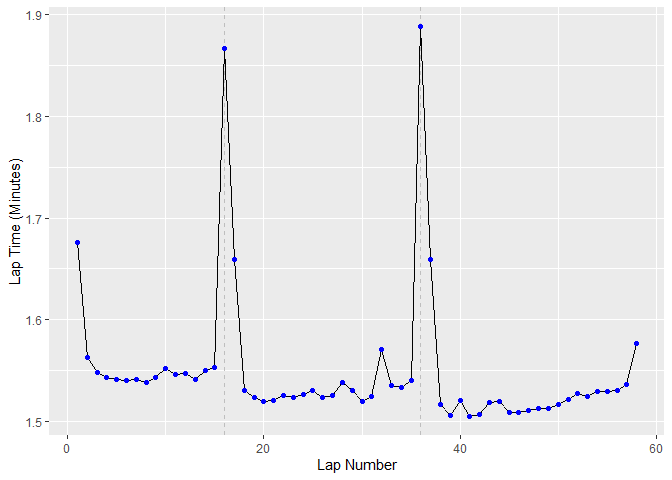
\includegraphics{dataProcessingDocument_files/figure-latex/lap and laptimes visualization for specific race and racer-1.pdf}

\begin{Shaded}
\begin{Highlighting}[]
\NormalTok{df_laptimes }\OperatorTok\StringTok{ }
\StringTok{  }\KeywordTok{filter}\NormalTok{(raceId }\OperatorTok{==}\StringTok{ }\DecValTok{841}\NormalTok{) }\OperatorTok\StringTok{ }
\StringTok{  }\KeywordTok{mutate}\NormalTok{(}\DataTypeTok{driverId =} \KeywordTok{as.factor}\NormalTok{(driverId))}\OperatorTok\StringTok{ }
\StringTok{  }\KeywordTok{ggplot}\NormalTok{(}\KeywordTok{aes}\NormalTok{(lap, milliseconds }\OperatorTok{/}\StringTok{ }\DecValTok{1000} \OperatorTok{/}\StringTok{ }\DecValTok{60}\NormalTok{)) }\OperatorTok{+}
\StringTok{  }\KeywordTok{geom_line}\NormalTok{(}\KeywordTok{aes}\NormalTok{(}\DataTypeTok{color =}\NormalTok{ driverId)) }\OperatorTok{+}\StringTok{ }
\StringTok{  }\KeywordTok{ylim}\NormalTok{(}\FloatTok{1.5}\NormalTok{, }\FloatTok{2.5}\NormalTok{) }\OperatorTok{+}\StringTok{ }
\StringTok{  }\KeywordTok{labs}\NormalTok{(}
    \DataTypeTok{x =} \StringTok{"Lap Number"}\NormalTok{,}
    \DataTypeTok{y =} \StringTok{"Lap Time (Minutes)"}
\NormalTok{  )}
\end{Highlighting}
\end{Shaded}

\begin{verbatim}
## Warning: Removed 1 row(s) containing missing values (geom_path).
\end{verbatim}

\includegraphics{dataProcessingDocument_files/figure-latex/lap number \& laptimes for all racers in a given race-1.pdf}

\end{document}
